\chapter{Results and Tests}\label{chap:Results}

\section{Validation}

Mavis' primary goal is to represent alignment similarity by color similarity. In order to validate our algorithm, we generated three sets of artificial similarity data and applied Mavis on them. Each data set contains a small number of similarity scores with simple patterns and trends. For simplicity, all the residues have been designated as gaps (`-'), because residue types do not affect the result of Mavis. The effectiveness of the algorithm is easily revealed in the coloring results, by comparing the color patterns with the original data trends.

The first data set consists of two sequences of length $21$. In the leftmost column, two residues have the highest similarity score, $1$; in the rightmost column, the lowest similarity score, $0$; in the other $19$ columns in between, the scores decrease from left to right in the step of $0.05$ (see Table \ref{tab:test_1}).

\begin{table}[htb]
\caption{Similarity Data Set for Validation Test \#1}\label{tab:test_1}\centering\small
\begin{tabular}{lccccccccccc} \toprule
  Columns           & 1   & 2    & 3   & 4    & 5   & 6    & 7   & 8    & 9   & 10   & 11  \\ \hline
  Sequence 1        & -   & -    & -   & -    & -   & -    & -   & -    & -   & -    & -   \\
  Sequence 2        & -   & -    & -   & -    & -   & -    & -   & -    & -   & -    & -   \\
  Similarity Score  & 1   & 0.95 & 0.9 & 0.85 & 0.8 & 0.75 & 0.7 & 0.65 & 0.6 & 0.55 & 0.5 \\ \bottomrule
\end{tabular}\vspace{4mm}
\begin{tabular}{lccccccccccc} \toprule
  Columns           & 12   & 13  & 14   & 15  & 16   & 17  & 18   & 19  & 20   & 21 \\ \hline
  Sequence 1        & -    & -   & -    & -   & -    & -   & -    & -   & -    & -  \\
  Sequence 2        & -    & -   & -    & -   & -    & -   & -    & -   & -    & -  \\
  Similarity Score  & 0.45 & 0.4 & 0.35 & 0.3 & 0.25 & 0.2 & 0.15 & 0.1 & 0.05 & 0  \\ \bottomrule
\end{tabular}
\end{table}

Figure \ref{fig:test_1} is the MSA matrix colored by Mavis. From left to right, the color difference between two sequences increases from very little to very significant in a gradual way. This result perfectly meets our expectation that the colors are not only representing the residue relationships within a column, but also rotated to become as smooth as possible within rows.

\begin{figure}[htb]
\center{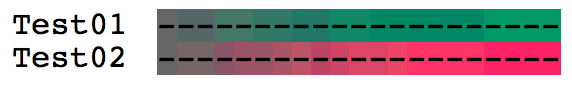
\includegraphics[width=0.6\textwidth]{figures/chap5_test_1.png}}
\caption[Coloring Result of Validation Test \#1]{The coloring result of validation test \#1.}\label{fig:test_1}
\end{figure}

The second data set is similar to the previous test, but consists of three sequences. Each column has three residues, of which any pair has the same similarity score. Similar to the first test, the scores decrease from $1$ on the left to $0$ on the right, in the step of $0.05$ (see Table \ref{tab:test_2}).

\begin{table}[htb]
\caption{Similarity Data Set for Validation Test \#2}\label{tab:test_2}\centering\small
\begin{tabular}{lccccccccccc} \toprule
  Columns                     & 1   & 2    & 3   & 4    & 5   & 6    & 7   & 8    & 9   & 10   & 11  \\ \hline
  Sequence 1                  & -   & -    & -   & -    & -   & -    & -   & -    & -   & -    & -   \\
  Sequence 2                  & -   & -    & -   & -    & -   & -    & -   & -    & -   & -    & -   \\
  Sequence 3                  & -   & -    & -   & -    & -   & -    & -   & -    & -   & -    & -   \\
  Similarity Score $s_{1,2}$  & 1   & 0.95 & 0.9 & 0.85 & 0.8 & 0.75 & 0.7 & 0.65 & 0.6 & 0.55 & 0.5 \\
  Similarity Score $s_{2,3}$  & 1   & 0.95 & 0.9 & 0.85 & 0.8 & 0.75 & 0.7 & 0.65 & 0.6 & 0.55 & 0.5 \\
  Similarity Score $s_{1,3}$  & 1   & 0.95 & 0.9 & 0.85 & 0.8 & 0.75 & 0.7 & 0.65 & 0.6 & 0.55 & 0.5 \\ \bottomrule
\end{tabular}\vspace{4mm}
\begin{tabular}{lccccccccccc} \toprule
  Columns                     & 12   & 13  & 14   & 15  & 16   & 17  & 18   & 19  & 20   & 21 \\ \hline
  Sequence 1                  & -    & -   & -    & -   & -    & -   & -    & -   & -    & -  \\
  Sequence 2                  & -    & -   & -    & -   & -    & -   & -    & -   & -    & -  \\
  Sequence 3                  & -    & -   & -    & -   & -    & -   & -    & -   & -    & -  \\
  Similarity Score $s_{1,2}$  & 0.45 & 0.4 & 0.35 & 0.3 & 0.25 & 0.2 & 0.15 & 0.1 & 0.05 & 0  \\
  Similarity Score $s_{2,3}$  & 0.45 & 0.4 & 0.35 & 0.3 & 0.25 & 0.2 & 0.15 & 0.1 & 0.05 & 0  \\
  Similarity Score $s_{1,3}$  & 0.45 & 0.4 & 0.35 & 0.3 & 0.25 & 0.2 & 0.15 & 0.1 & 0.05 & 0  \\ \bottomrule
\end{tabular}
\end{table}

Figure \ref{fig:test_2} is the MSA matrix of the second test. Similarly, the color differences between any pair of the three sequences gradually increase from very little on the left to very significant on the right. In addition to the expectation of preserving residue distances and color rotation, this figure also illustrates how color flipping affects the result. For comparison, Figure \ref{fig:test_2a} is the result from the same data set, but the flipping optimization is manually disabled. Obviously, colors in a few columns are not be able to match adjacent ones. The coordinates of these three residues are arranged in the two-dimensional color space as an isosceles triangle, in which the three vertices may be clockwise or counterclockwise. If both situations exist in this MSA matrix, their color patterns can not match, no matter how they are rotated. 

\begin{figure}[htb]
\center{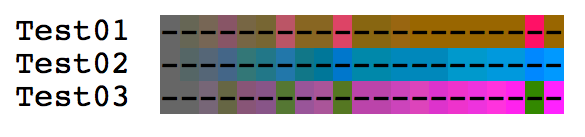
\includegraphics[width=0.6\textwidth]{figures/chap5_test_2a.png}}
\caption[Coloring Result of Validation Test \#2 without Flipping]{The coloring result of validation test \#2 without color flipping.}\label{fig:test_2a}
\end{figure}

\begin{figure}[htb]
\center{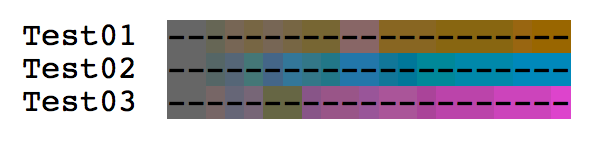
\includegraphics[width=0.6\textwidth]{figures/chap5_test_2.png}}
\caption[Coloring Result of Validation Test \#2 with Flipping]{The coloring result of validation test \#2 with color flipping.}\label{fig:test_2}
\end{figure}

The third data set consists of four sequences, which are divided into two groups. Within each column, any two residues from the same group have the maximum similarity score, meaning that they are exactly the same; any two residues from different groups have the same similarity score. Similarly, the scores decrease from $1$ on the left to $0$ on the right, in the same way as the first and second tests (see Table \ref{tab:test_3}).

\begin{table}[htb]
\caption{Similarity Data Set for Validation Test \#3}\label{tab:test_3}\centering\small
\begin{tabular}{lccccccccccc} \toprule
  Columns                     & 1   & 2    & 3   & 4    & 5   & 6    & 7   & 8    & 9   & 10   & 11  \\ \hline
  Sequence 1 (Group 1)        & -   & -    & -   & -    & -   & -    & -   & -    & -   & -    & -   \\
  Sequence 2 (Group 1)        & -   & -    & -   & -    & -   & -    & -   & -    & -   & -    & -   \\
  Sequence 3 (Group 2)        & -   & -    & -   & -    & -   & -    & -   & -    & -   & -    & -   \\
  Sequence 4 (Group 2)        & -   & -    & -   & -    & -   & -    & -   & -    & -   & -    & -   \\
  Similarity Scores \\
  $s_{1,2}$ and $s_{3,4}$     & 0   & 0    & 0   & 0    & 0   & 0    & 0   & 0    & 0   & 0    & 0   \\
  Similarity Scores \\
  $s_{1,3}$, $s_{1,4}$, $s_{2,3}$ and $s_{2,4}$
                              & 1   & 0.95 & 0.9 & 0.85 & 0.8 & 0.75 & 0.7 & 0.65 & 0.6 & 0.55 & 0.5 \\ \bottomrule
\end{tabular}\vspace{4mm}
\begin{tabular}{lcccccccccc} \toprule
  Columns                     & 12   & 13  & 14   & 15  & 16   & 17  & 18   & 19  & 20   & 21 \\ \hline
  Sequence 1 (Group 1)        & -    & -   & -    & -   & -    & -   & -    & -   & -    & -  \\
  Sequence 2 (Group 1)        & -    & -   & -    & -   & -    & -   & -    & -   & -    & -  \\
  Sequence 3 (Group 2)        & -    & -   & -    & -   & -    & -   & -    & -   & -    & -  \\
  Sequence 4 (Group 2)        & -    & -   & -    & -   & -    & -   & -    & -   & -    & -  \\
  Similarity Scores \\
  $s_{1,2}$ and $s_{3,4}$     & 0    & 0   & 0.35 & 0.3 & 0.25 & 0.2 & 0.15 & 0.1 & 0.05 & 0  \\
  Similarity Scores \\
  $s_{1,3}$, $s_{1,4}$, $s_{2,3}$ and $s_{2,4}$
                              & 0.45 & 0.4 & 0.35 & 0.3 & 0.25 & 0.2 & 0.15 & 0.1 & 0.05 & 0  \\ \bottomrule
\end{tabular}
\end{table}

The result of this data set is shown in Figure \ref{fig:test_3}. First, each sequence has the correct gradient color pattern. Second, sequences from different groups are colored in different hues, reflecting the alignment distances between groups. Third, sequences from the same group share the same color pattern, reflecting the zero distances within a group. This result shows that Mavis is capable of handling more complex situations.

\begin{figure}[htb]
\center{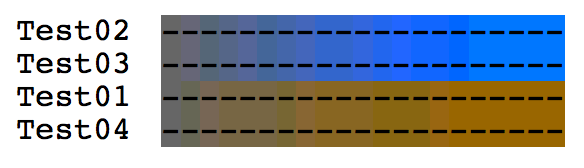
\includegraphics[width=0.6\textwidth]{figures/chap5_test_3.png}}
\caption[Coloring Result of Validation Test \#3]{The coloring result of validation test \#3.}\label{fig:test_3}
\end{figure}

% \section{Benchmarks}
% 
% In order to assess the performance of our approach, we run Mavis on a number of real data sets and recorded the amount of time taken by Mavis to complete color generation, color optimization, and other visualization steps.
% 
% We used the classical alignment data set, \emph{BALIBASE} versions 3.0. Benchmark Alignment dataBASE (BALIBASE) is a database constructed to provide documented, manually refined, high-quality multiple sequence alignments. It has been adopted by many algorithms to evaluate the alignment quality. Here we adopted the latest version 3.0 to evaluate the performance of Mavis \cite{Thompson:2005fk}.
% 
% \emph{(Under Construction)}
